


\documentclass[compress,t]{beamer}

\usetheme{hsrm}


\usepackage[utf8]{inputenc}
\usepackage[german]{babel}
\usepackage{graphicx}
\usepackage{multicol}
\usepackage{tabularx,ragged2e}
\usepackage{booktabs}
\usepackage{listings}

\usepackage{hhline}
\usepackage{multirow}

\usepackage{color}

%--------------------------------------------------------------------------
% General presentation settings
%--------------------------------------------------------------------------
\title{Privacy Ranking}
\subtitle{Wahlprojekt}
\date{Letztes Update: \today}
\author{Max Mustermann}
\institute{Studienbereich Informatik\\Hochschule {RheinMain}}

\lstset{
  frame=single,
  basicstyle={\small\ttfamily},
  aboveskip=3mm,
  belowskip=3mm,
  breaklines=true,
  breakatwhitespace=true,
  tabsize=4,
  escapeinside={(*@}{@*)}
}

\begin{document}

\maketitle


%--------------------------------------------------------------------------
% Table of contents
%--------------------------------------------------------------------------
\section*{Gliederung}
\begin{frame}{Gliederung}
    \tableofcontents[hideallsubsections]
\end{frame}


%--------------------------------------------------------------------------
% Content
%--------------------------------------------------------------------------
\section{Einführung or whatever}

\begin{frame}
    Alles was wir am Anfang erzählen wollen
\end{frame}

\section{Unsere App}

\begin{frame}
    Unsere App halt
\end{frame}

\section{Webservice}

\begin{frame}
    Webservice
\end{frame}

\section{Wie kommen wir an die Daten?}

\begin{frame}{Website Google Playstore}

    \begin{center}
        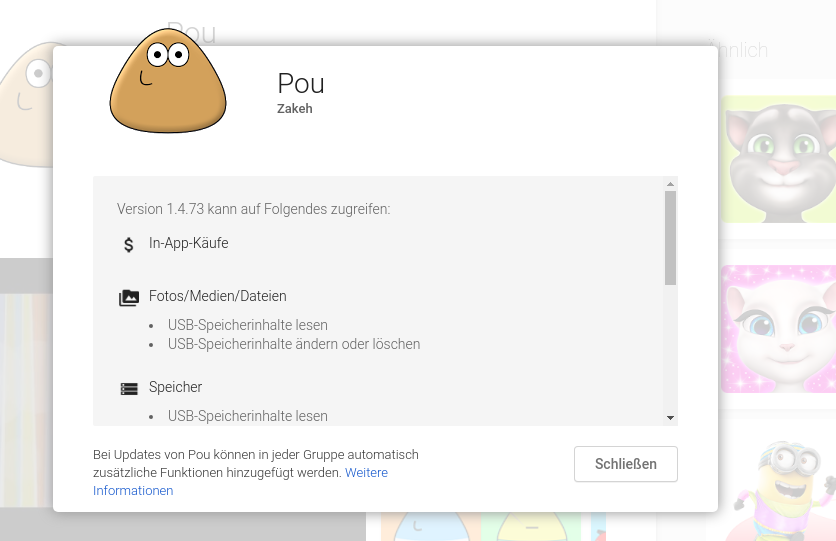
\includegraphics[width=0.6\textwidth]{img/google_play.png}
        \newline
        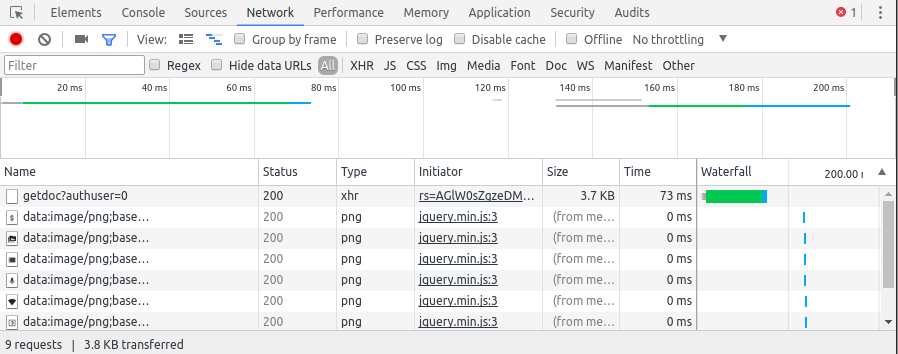
\includegraphics[width=0.6\textwidth]{img/google_play_network.png}
    \end{center}

\end{frame}

\begin{frame}[fragile]{Scraping der Daten}

    \begin{itemize}
        \item Zugriff auf den Webservice von Google
        \item https://play.google.com/store/xhr/getdoc?authuser=0
        \item POST (ids=app\_id, xhr=1)
    \end{itemize}

    \begin{lstlisting}
[["gdar",1,[["me.pou.app","me.pou.app",1,3,
"/store/apps/details?id\u003dme.pou.app",
"/store/apps/details?id\u003dme.pou.app",
"https://play.google.com/store/apps/details
?id\u003dme.pou.app","https://market.android
.com/details?id\u003dme.pou.app","Pou",...
    \end{lstlisting}

\end{frame}

\begin{frame}[fragile]{Extrahieren der Daten}
    \begin{itemize}
        \item Schreiben eines Wrappers in Python
        \item Lokalisieren der nötigen Informationen
    \end{itemize}

    \begin{lstlisting}[language=Python]
def extract_title(data):
    return _remove_emojis(data[0][2][0][8])

def extract_description(data):
    return _remove_emojis(data[0][2][0][9])

def extract_rating(data):
    return data[0][2][0][23]
    \end{lstlisting}

\end{frame}

\section{Datenbank}

\begin{frame}{MariaDB Datenbank}

    \begin{center}
        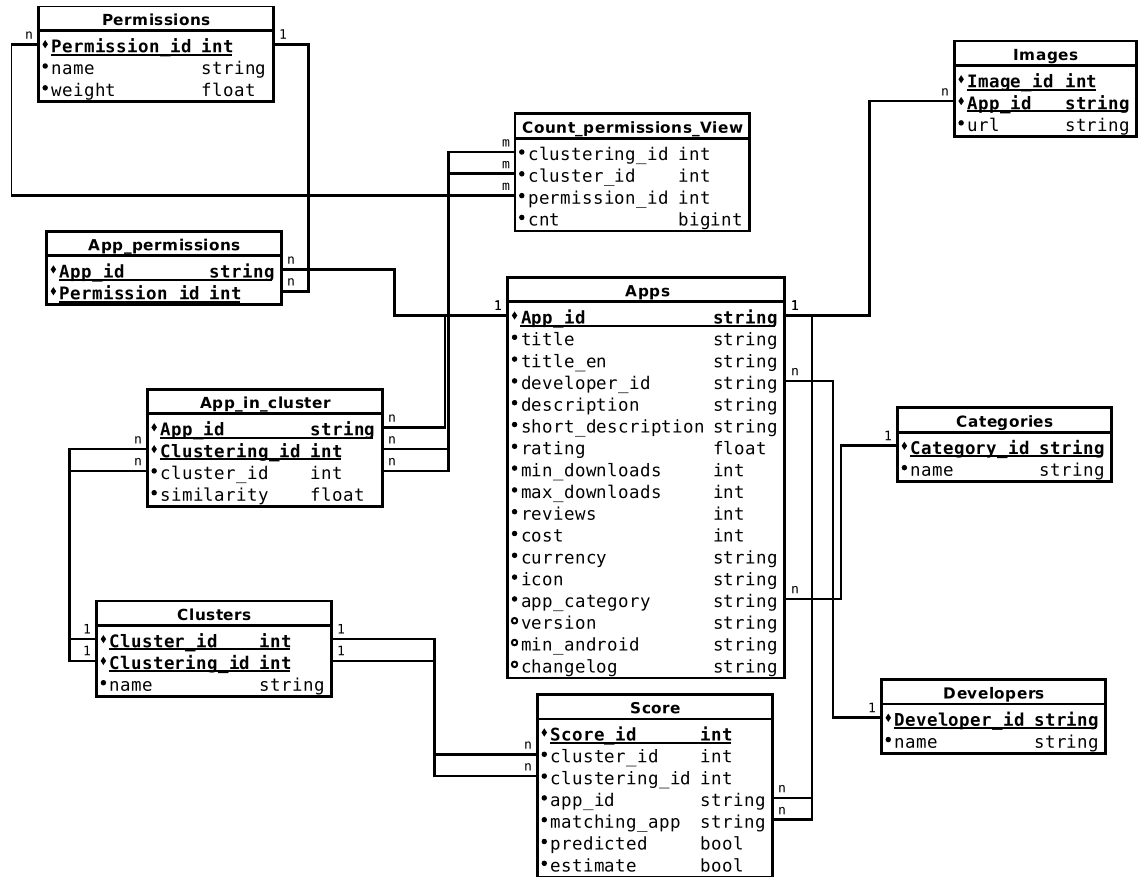
\includegraphics[width=0.9\textwidth]{img/Scheme_extended_3.png}
    \end{center}

\end{frame}

\begin{frame}[fragile]{Stored procedure}

    \begin{lstlisting}[language=SQL]
DELIMITER $$
DROP FUNCTION IF EXISTS countAppsInCluster$$
CREATE FUNCTION countAppsInCluster( c_id INT, cing_id INT )
RETURNS INT DETERMINISTIC
READS SQL DATA
BEGIN
    DECLARE cnt INT;
    SELECT count(App_id) INTO cnt FROM App_in_cluster WHERE cluster_id = c_id
        AND Clustering_id = cing_id;
    RETURN cnt;
END$$
DELIMITER ;
    \end{lstlisting}

    \textcolor{red}{\(\Rightarrow\)} Schlechte Idee, imperformant!

\end{frame}

\section{Kategorisierung und Bewertung der Apps}

\begin{frame}{Datamining}

    \begin{itemize}
        \item Kategorisierung mithilfe von Clustering
        \item Auswahl zwischen den einzelnen Algorithmen
            \begin{itemize}
                \item K-Means
                    \begin{itemize}
                        \item Anzahl Cluster muss bekannt sein
                    \end{itemize}
                \item Affinity propagation
                    \begin{itemize}
                        \item Terminiert nicht
                    \end{itemize}
                \item Mean-Shift
                    \begin{itemize}
                        \item Terminiert nicht
                    \end{itemize}
                \item Ward hierarchical clustering
                    \begin{itemize}
                        \item Terminiert nicht
                    \end{itemize}
                \item DBSCAN
                    \begin{itemize}
                        \item Rauschen
                    \end{itemize}
            \end{itemize}
    \end{itemize}

\end{frame}

\begin{frame}{DBSCAN}

    \begin{center}
        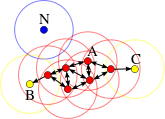
\includegraphics[width=0.4\textwidth]{img/dbscan.png}{Quelle: \href{http://www.oracle.com/technetwork/java/javase/tech/memorymanagement-whitepaper-1-150020.pdf}{Wikipedia}}
    \end{center}

    \begin{itemize}
        \item Density-based spatial clustering of applications with noise
        \item Abstand (Epsilon) muss gut gewählt werden
    \end{itemize}

\end{frame}

\begin{frame}{TF-IDF}

    \begin{itemize}
        \item Clustering-Algorithmen funktionieren nur mit numerischen Werten
        \item Text frequenzy
            \begin{itemize}
                \item Je häufiger Wort in Text enthalten \(\Rightarrow\) bedeutend
                \item Wert für \emph{min-df} muss gut gewählt werden
            \end{itemize}
        \item Inversed document frequenzy
            \begin{itemize}
                \item Je häufiger Wort in allen Dokumenten enthalten \(\Rightarrow\) unbedeutend
                \item Wert für \emph{max-df} muss gut gewählt werden
            \end{itemize}
        \item Dadurch entsteht Documents \(\times\) Features Matrix
        \item Max. Feautures werden bestimmt.
    \end{itemize}

\end{frame}

\begin{frame}{Gute Metric finden}

    \begin{columns}[t]
        \column{.5\textwidth}
        \centering
        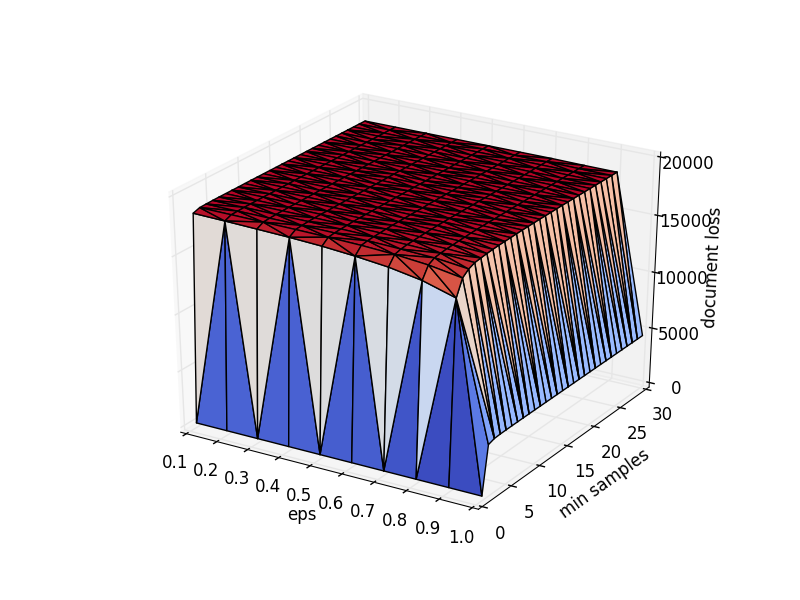
\includegraphics[width=0.8\textwidth]{img/1_euclidian.png}{Euclidian}\\
        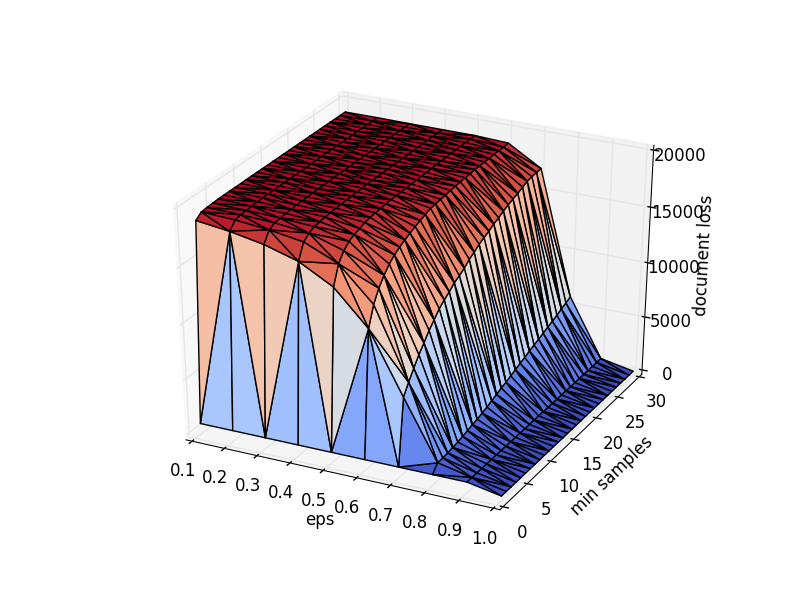
\includegraphics[width=0.8\textwidth]{img/2_cosine_brute.png}{Cosine}
        \column{.5\textwidth}
        \centering
        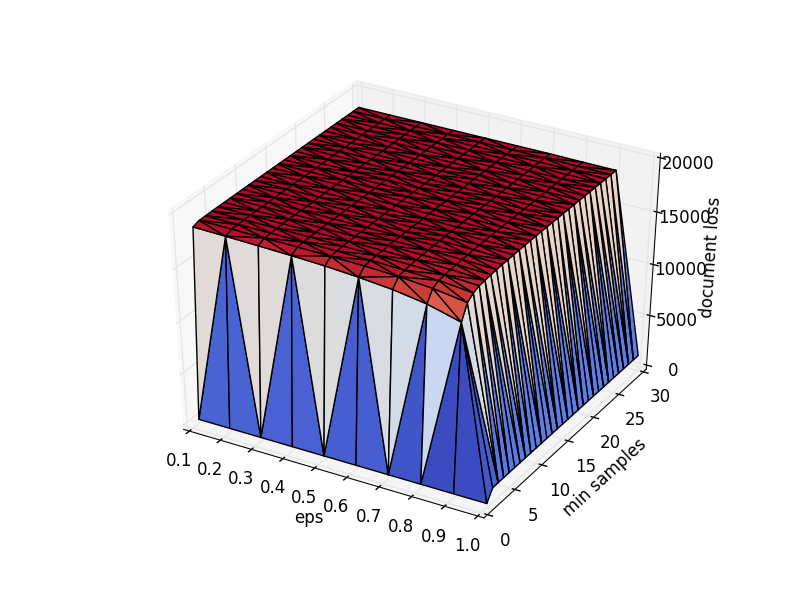
\includegraphics[width=0.8\textwidth]{img/3_l2.png}{L2}\\
        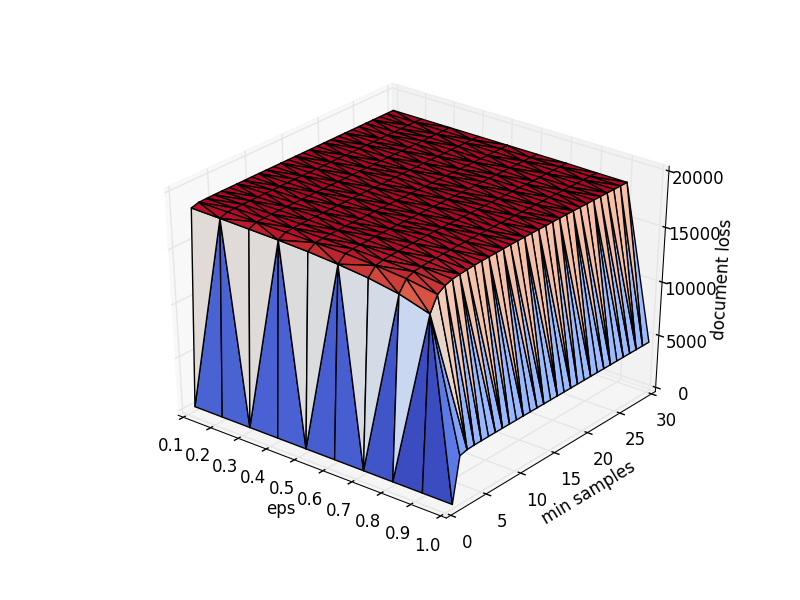
\includegraphics[width=0.8\textwidth]{img/4_minkowski_p_2_0.png}{Minkowski}
    \end{columns}

\end{frame}

\begin{frame}{Gute Parameter finden - Testdaten}

    \begin{columns}[t]
        \column{.5\textwidth}
        \centering
        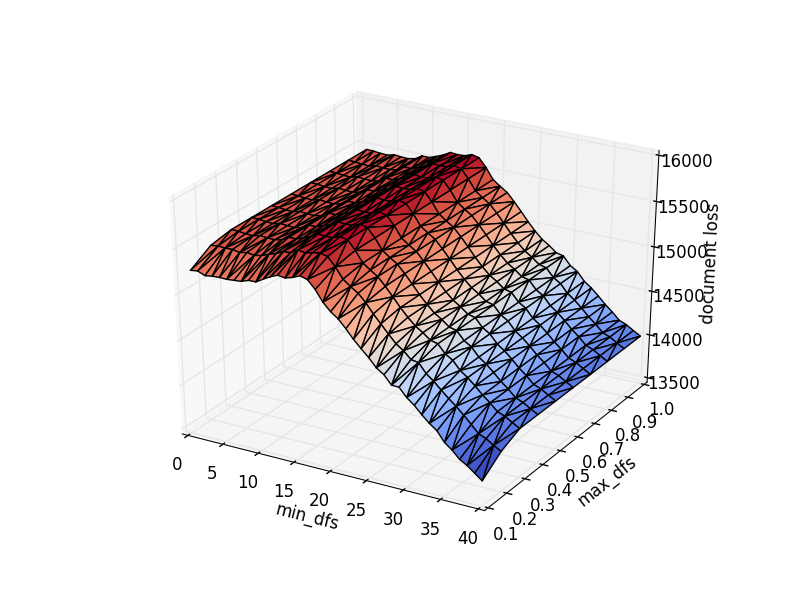
\includegraphics[width=1.0\textwidth]{img/df_3_cosin.png}\\
        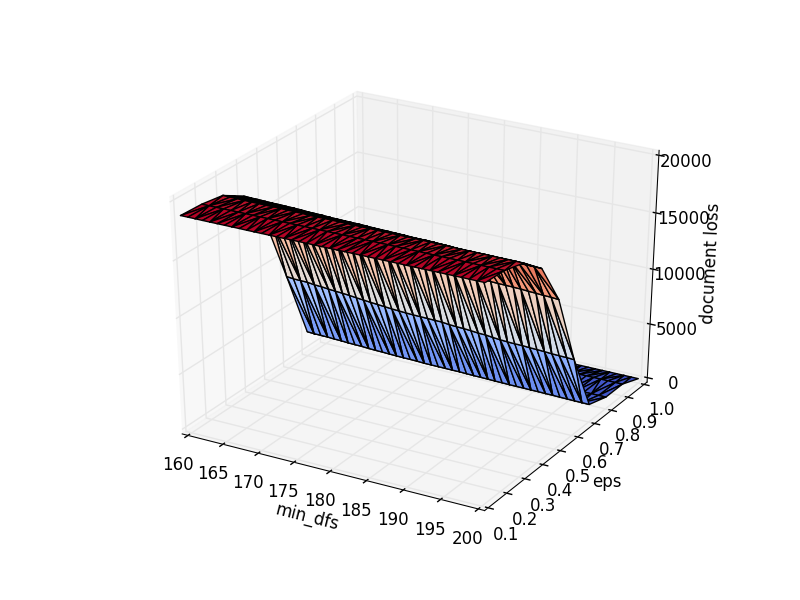
\includegraphics[width=1.0\textwidth]{img/df_eps_1_cosin.png}
        \column{.5\textwidth}
        \centering
        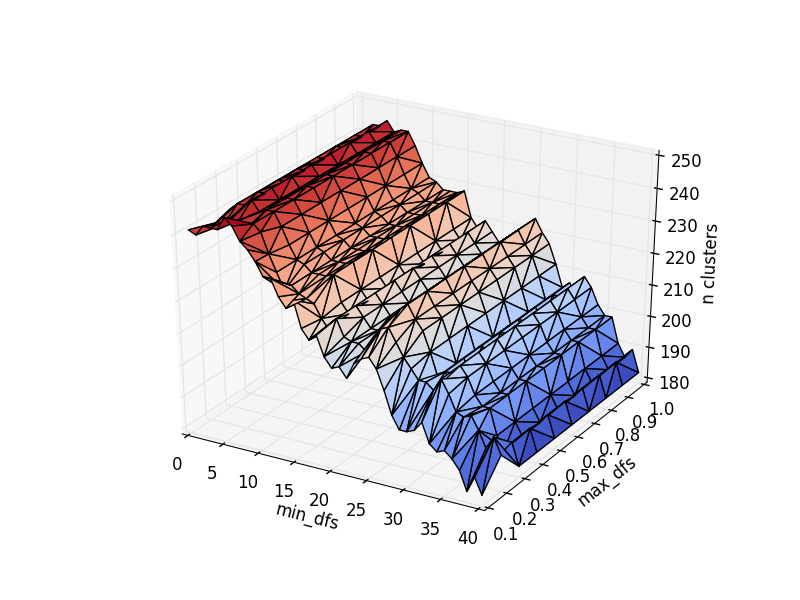
\includegraphics[width=1.0\textwidth]{img/df_3_cosin_nofc.png}\\
        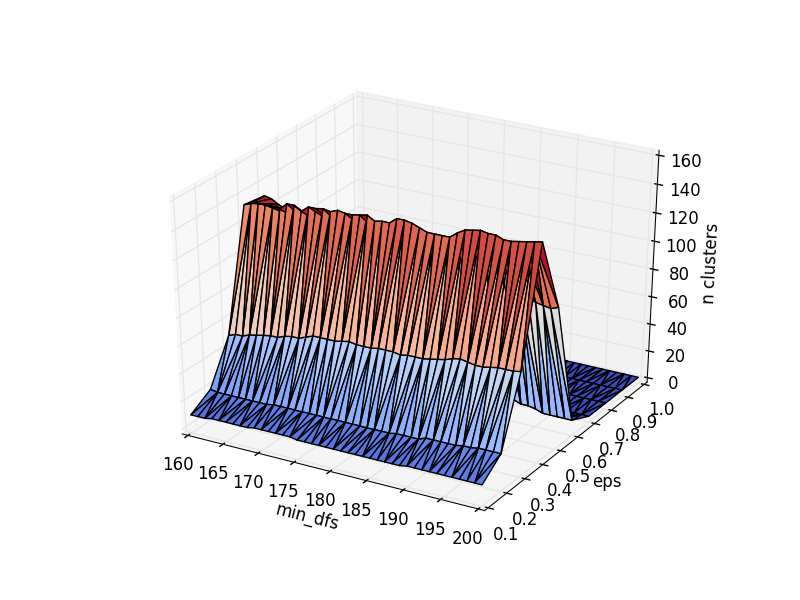
\includegraphics[width=1.0\textwidth]{img/df_eps_1_cosin_nofc.png}
    \end{columns}

\end{frame}

\begin{frame}{Gute Parameter finden - Google Play Daten}

    \begin{columns}[t]
        \column{.5\textwidth}
        \centering
        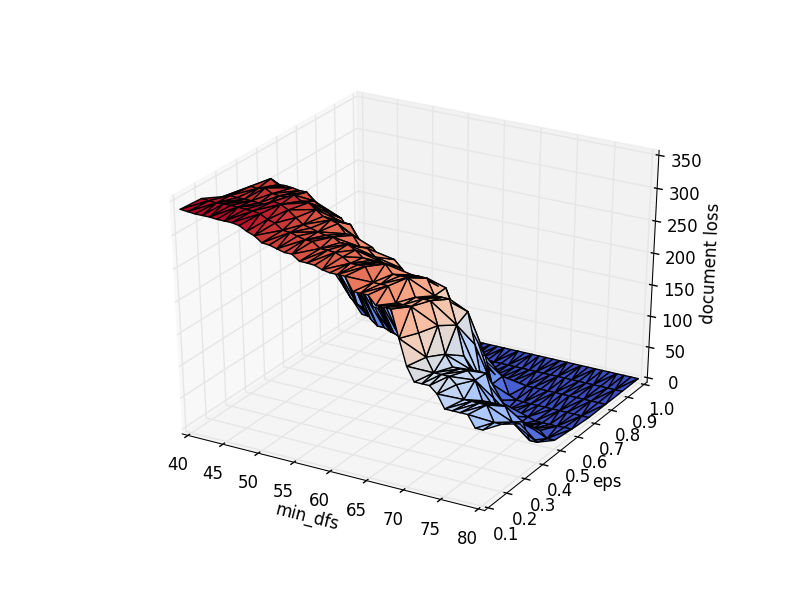
\includegraphics[width=1.0\textwidth]{img/gp_2_cosin.png}\\
        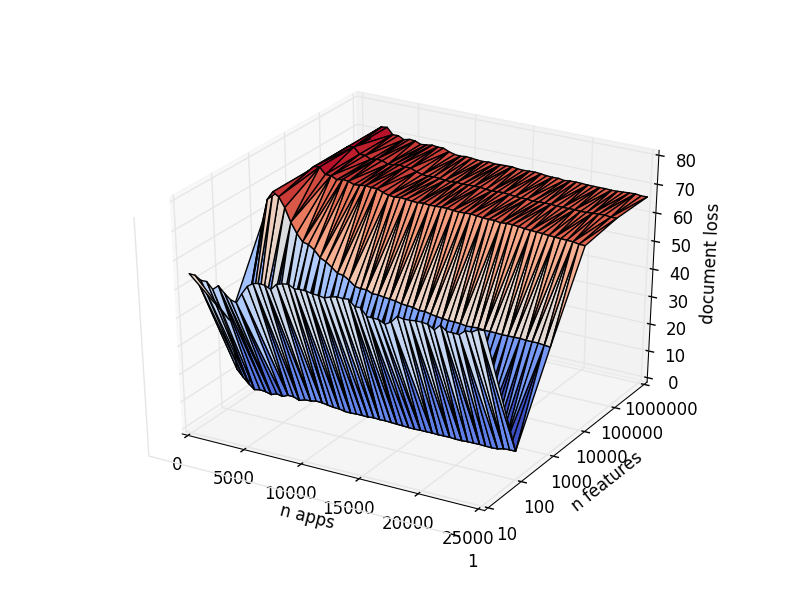
\includegraphics[width=1.0\textwidth]{img/features_3.png}
        \column{.5\textwidth}
        \centering
        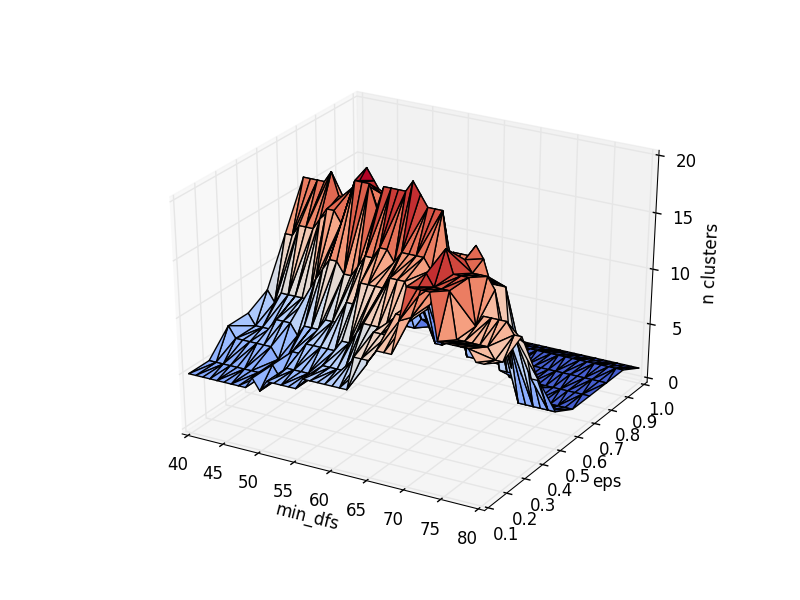
\includegraphics[width=1.0\textwidth]{img/gp_2_cosin_nofc.png}\\
        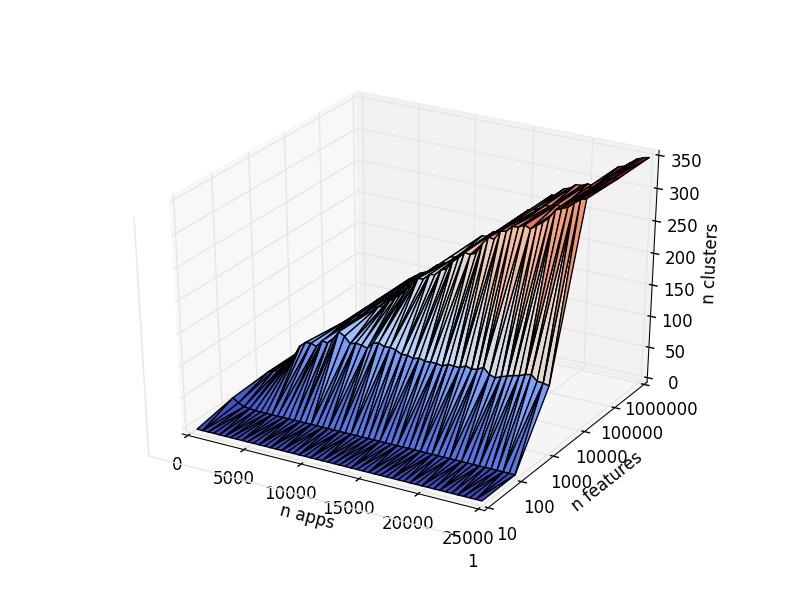
\includegraphics[width=1.0\textwidth]{img/features_3_nofc.png}
    \end{columns}

\end{frame}

\begin{frame}{Gute Parameter finden}

    \begin{itemize}
        \item max-df: 0.01
        \item min-df: 0.005
        \item eps: 0.45
        \item min-samples: 30
        \item features: 1500
    \end{itemize}

    \textcolor{green}{\(\Rightarrow\)} 42 Cluster\\
    \textcolor{red}{\(\Rightarrow\)} Mehr als 50\% Rauschen\\
    \textcolor{red}{\(\Rightarrow\)} 1 Cluster viel zu groß

\end{frame}

\begin{frame}{Kombination mit anderen Algorithmen}

    \begin{itemize}
        \item K-Means
            \begin{itemize}
                \item Anzahl Cluster aus DBSCAN \(\rightarrow\) \textcolor{orange}{mäßiger} Erfolg
                \item Anzahl GP Kategorien \(\rightarrow\) \textcolor{orange}{mäßiger} Erfolg
            \end{itemize}
        \item Classifier
            \begin{itemize}
                \item DecisionTree \(\rightarrow\) \textcolor{red}{mieserabler} Erfolg
                \item BernoulliNB \(\rightarrow\) \textcolor{red}{mieserabler} Erfolg
                \item MLP \(\rightarrow\) \textcolor{red}{mieserabler} Erfolg
                \item AdaBoost \(\rightarrow\) \textcolor{red}{mieserabler} Erfolg
                \item KNeighbors  \(\rightarrow\) \textcolor{green}{akzeptabler} Erfolg
            \end{itemize}
    \end{itemize}

    \textcolor{green}{\(\Rightarrow\)} Kein Verlust mehr durch Rauschen\\
    \textcolor{red}{\(\Rightarrow\)} Zu großer Cluster wurde noch größer\\
    \textcolor{red}{\(\Rightarrow\)} Cluster beinhaltet mehr als 50\% apps

\end{frame}

\begin{frame}{Hierarchical DBSCAN}

    Aufteilung von zu großen Cluster in kleinere.

    \textcolor{red}{\(\Rightarrow\)} Sprengt den Arbeitsspeicher.
    \begin{quote}
        Dies liegt an der mieserablen Implementierung in SKLearn.
        Es ist besser, wenn du's selbst implementierst.\\
        - Viele Leute bei Stackoverflow
    \end{quote}

    Eigene Variante in Kombination mit KNeighbors:
    \begin{itemize}
        \item Zu große Cluster werden erneut mit DBSCAN geclustert (kleineres Epsilon)
        \item Dabei entstandendes Rauschen wird mithilfe KNeighbors neu verteilt
    \end{itemize}

    \textcolor{red}{\(\Rightarrow\)} Clusterqualität wurde schlechter, kein guter Erfolg

\end{frame}

\begin{frame}{Bewertung der Apps}

    Die Apps werden nach dem Einfluss auf die Privatsphäre bewertet.

    \begin{enumerate}
        \item Sammeln der Berechtigungen innerhalb eines Clusters
    \end{enumerate}

    \begin{center}
    \begin{tabular}{|*{6}{c|}}
        \multicolumn{6}{c}{Permissions} \tabularnewline
        %\cline{2-10}
        \hline
        \textbf{0} & \textbf{4} & \textbf{9} & \textbf{10} & \textbf{11} & \textbf{12} \\
        \hline
    \end{tabular}
    \end{center}

    Mit den Berechtigungen:
    \begin{center}
    \begin{tabular}{ | c | l | }
        \hline
        \textbf{ID} & \textbf{Name} \\
        \hline
        0 & In-App-Purchases \\
        4 & Calender \\
        9 & Pictures/Media/Files \\
        10 & Storage \\
        11 & Camera \\
        12 & Microphone \\
        \hline
    \end{tabular}
    \end{center}

\end{frame}

\begin{frame}{Bewertung der Apps}

    \begin{enumerate}
        \setcounter{enumi}{1}
        \item Berechnung der Gewichtung
    \end{enumerate}

    Besteht aus zwei Teilen:
    \begin{itemize}
        \item Relative häufigkeit von App die diese Berechtigung \textbf{nicht} haben
    \end{itemize}

    \begin{center}
    \begin{tabular}{|*{6}{c|}}
        %\cline{2-10}
        \hline
        0.4 & 0.8 & 0.6 & 0.2 & 0.0 & 0.6 \\
        \hline
    \end{tabular}
    \end{center}

    \begin{itemize}
        \item Bösheit der Berechtigung
    \end{itemize}

    \begin{center}
    \begin{tabular}{|*{6}{c|}}
        %\cline{2-10}
        \hline
        0.1 & 0.6 & 0.1 & 0.1 & 0.9 & 0.9 \\
        \hline
    \end{tabular}
    \end{center}

\end{frame}

\begin{frame}{Bewertung der Apps}

    Diese werden miteinander multipliziert.

    \begin{center}
    \begin{tabular}{|*{6}{c|}}
        \multicolumn{6}{c}{Permissions} \tabularnewline
        %\cline{2-10}
        \hline
        \textbf{0} & \textbf{4} & \textbf{9} & \textbf{10} & \textbf{11} & \textbf{12} \\
        \hline{}
        0.04 & 0.48 & 0.06 & 0.02 & 0.0 & 0.54 \\
        \hline
    \end{tabular}
    \end{center}

    \begin{enumerate}
        \setcounter{enumi}{2}
        \item Füllen der Matrix
    \end{enumerate}

      \begin{center}
      \begin{tabular}{c|c||*{6}{c|}}
        \multicolumn{2}{c}{} & \multicolumn{6}{c}{Permissions} \tabularnewline
        \cline{2-8}
        \multirow{6}*{\rotatebox{90}{Apps}} & ID
    &    \textbf{0} & \textbf{4} & \textbf{9} & \textbf{10} & \textbf{11} & \textbf{12}  \tabularnewline[0 ex]
    %\cline{2-8}
    \hhline{~|=||=|=|=|=|=|=|}
    &    \bfseries 14 & 0.04 & 0.0 & 0.0 & 0.02 & 0.0 & 0.54 \tabularnewline [0 ex]
        \cline{2-8}
    &    \bfseries 42 & 0.0 & 0.48 & 0.06 & 0.0 & 0.0 & 0.0 \tabularnewline [0 ex]
        \cline{2-8}
    &    \bfseries 145 & 0.04 & 0.0 & 0.0 & 0.02 & 0.0 & 0.0 \tabularnewline [0 ex]
        \cline{2-8}
    &    \bfseries 465 & 0.04 & 0.0 & 0.06 & 0.02 & 0.0 & 0.54 \tabularnewline [0 ex]
        \cline{2-8}
    &    \bfseries 1010 & 0.0 & 0.0 & 0.0 & 0.02 & 0.0 & 0.0 \tabularnewline [0 ex]
        \cline{2-8}
      \end{tabular}
      \end{center}

\end{frame}

\begin{frame}{Bewertung der Apps}

    \begin{enumerate}
        \setcounter{enumi}{3}
        \item Aufsummieren der Werte
    \end{enumerate}

      \begin{center}
      \begin{tabular}{c|c||*{6}{c|}|c|}
        \multicolumn{2}{c}{} & \multicolumn{6}{c}{Permissions} & \multicolumn{1}{c}{} \tabularnewline
        \cline{2-9}
        \multirow{6}*{\rotatebox{90}{Apps}} & ID
    &    \textbf{0} & \textbf{4} & \textbf{9} & \textbf{10} & \textbf{11} & \textbf{12} & \(\sum\)  \tabularnewline[0 ex]
    %\cline{2-9}
    \hhline{~|=||=|=|=|=|=|=||=|}
    &    \bfseries 14 & 0.04 & 0.0 & 0.0 & 0.02 & 0.0 & 0.54 & \textbf{0.6} \tabularnewline [0 ex]
        \cline{2-9}
    &    \bfseries 42 & 0.0 & 0.48 & 0.06 & 0.0 & 0.0 & 0.0 & \textbf{0.54} \tabularnewline [0 ex]
        \cline{2-9}
    &    \bfseries 145 & 0.04 & 0.0 & 0.0 & 0.02 & 0.0 & 0.0 & \textbf{0.06} \tabularnewline [0 ex]
        \cline{2-9}
    &    \bfseries 465 & 0.04 & 0.0 & 0.06 & 0.02 & 0.0 & 0.54 & \textbf{0.66} \tabularnewline [0 ex]
        \cline{2-9}
    &    \bfseries 1010 & 0.0 & 0.0 & 0.0 & 0.02 & 0.0 & 0.0 & \textbf{0.02} \tabularnewline [0 ex]
        \cline{2-9}
      \end{tabular}
      \end{center}

\end{frame}

\begin{frame}[fragile]{Bewertung der Apps}

    \begin{enumerate}
        \setcounter{enumi}{4}
        \item Aufteilen in 3 Gruppen mithilfe K-Means
    \end{enumerate}

    \begin{columns}
        \begin{column}{0.5\textwidth}
              \begin{center}
                  \begin{tabular}{c|c|c|}
                    %\multicolumn{2}{c}{} & \multicolumn{6}{c}{Permissions} & \multicolumn{1}{c}{} \tabularnewline
                    \cline{2-3}
                    \multirow{6}*{\rotatebox{90}{Apps}} & ID
                &  \(\sum\) \tabularnewline[0 ex]
                %\cline{2-3}
                \hhline{~|=|=|}
                &    \bfseries \color{red} 14 & \color{red} 0.6 \tabularnewline [0 ex]
                    \cline{2-3}
                &    \bfseries \color{yellow} 42 & \color{yellow} 0.54 \tabularnewline [0 ex]
                    \cline{2-3}
                &    \bfseries \color{green} 145 & \color{green} 0.06 \tabularnewline [0 ex]
                    \cline{2-3}
                &    \bfseries \color{red} 465 & \color{red} 0.66 \tabularnewline [0 ex]
                    \cline{2-3}
                &    \bfseries \color{green} 1010 & \color{green} 0.02 \tabularnewline [0 ex]
                    \cline{2-3}
                  \end{tabular}
              \end{center}
        \end{column}
        \begin{column}{0.5\textwidth} %%
            \begin{itemize}
                \item Gut - Grün
                    \begin{itemize}
                        \item 80 - 120 degree
                    \end{itemize}
                \item Mittel - Gelb
                    \begin{itemize}
                        \item 30 - 79 degree
                    \end{itemize}
                \item Schlecht - Rot
                    \begin{itemize}
                        \item 0 - 29 degree
                    \end{itemize}
            \end{itemize}
        \end{column}
    \end{columns}

    \begin{lstlisting}[language=Python]
# 0 - 100
value = 100 - ((app_values[i] - min_value) * 100.0) / (max_value - min_value)
# min_range - max_range
value = (value * (color_range[1] - color_range[0]) / 100) + color_range[0]
    \end{lstlisting}

\end{frame}

\end{document}


"""
red 0 degree - 29 degree
yellow 30 degree - 79 degree
green 80 degree - 120 degree
"""




